\ifx\mainfile\undefined
%  ========================================================================
%  Copyright (c) 2006-2011 The University of Washington
%
%  Licensed under the Apache License, Version 2.0 (the "License");
%  you may not use this file except in compliance with the License.
%  You may obtain a copy of the License at
%
%      http://www.apache.org/licenses/LICENSE-2.0
%
%  Unless required by applicable law or agreed to in writing, software
%  distributed under the License is distributed on an "AS IS" BASIS,
%  WITHOUT WARRANTIES OR CONDITIONS OF ANY KIND, either express or implied.
%  See the License for the specific language governing permissions and
%  limitations under the License.
%  ========================================================================
%
 
\documentclass [11pt, twoside] {uwthesis}

\usepackage{color}
\usepackage{url}
\usepackage{amsmath}
\usepackage{amsfonts}
\usepackage[bookmarks,
	hidelinks,
	plainpages=false,
	pdfpagelabels,
	pagebackref=true,
            ]{hyperref}
\renewcommand*{\backref}[1]{}% for backref < 1.33 necessary
\renewcommand*{\backrefalt}[4]{%
  \ifcase #1 %
    (No citations.)%
  \or
    (Cited on page #2.)%
  \else
    (Cited on pages #2.)%
  \fi
}

\newcommand{\biburl}[1]{{\tt<}\url{#1}{\tt>}}

\hypersetup{%
pdfauthor = {Daniel Chaim Halperin},
pdftitle = {Simplifying the Configuration of 802.11 Wireless Networks with Effective SNR},
pdfsubject = {Ph.D. Dissertation},
pdfkeywords = {},
pdfcreator = {University of Washington, Computer Science and Engineering},
pdfproducer = {},
bookmarksopen = {true},
pdfpagelayout = {TwoColumnRight},
}

\usepackage{footnotebackref}
%%%%%%%%%%%%%%%%%%%%%%%%%%%%%%%%%%%%%%%%%%%%%%%%%%%%%%
%%%        Formatting sections                     %%%
%%%%%%%%%%%%%%%%%%%%%%%%%%%%%%%%%%%%%%%%%%%%%%%%%%%%%%
\newcommand{\algref}[1]{Algorithm~\ref{#1}}
\newcommand{\chapref}[1]{Chapter~\ref{#1}}
\renewcommand{\eqref}[1]{Equation~\ref{#1}}
\newcommand{\figref}[1]{Figure~\ref{#1}}
\newcommand{\secref}[1]{\S\ref{#1}}
\newcommand{\tabref}[1]{Table~\ref{#1}}
\newcommand{\heading}[1]{\vspace{4pt}\noindent\textbf{#1}}
\newcommand{\topheading}[1]{\noindent\textbf{#1}}
\newcommand{\noheading}[0]{\vspace{4pt}\noindent}

%%%%%%%%%%%%%%%%%%%%%%%%%%%%%%%%%%%%%%%%%%%%%%%%%%%%%%
%%%        XXX and other warnings                  %%%
%%%%%%%%%%%%%%%%%%%%%%%%%%%%%%%%%%%%%%%%%%%%%%%%%%%%%%
\newcommand{\xxx}[1]{\textit{\color{red}XXX #1}}

%%%%%%%%%%%%%%%%%%%%%%%%%%%%%%%%%%%%%%%%%%%%%%%%%%%%%%
%%%        Units                                   %%%
%%%%%%%%%%%%%%%%%%%%%%%%%%%%%%%%%%%%%%%%%%%%%%%%%%%%%%
\usepackage{xspace}
\newcommand{\unitsep}{\texorpdfstring{\,}{ }}
\def\unit#1{% from: http://www.tex.ac.uk/cgi-bin/texfaq2html?label=csname "Defining a macro from an argument"
  \expandafter\def\csname #1\endcsname{\unitsep\text{#1}\xspace}%
}
\def\varunit#1#2{% from: http://www.tex.ac.uk/cgi-bin/texfaq2html?label=csname "Defining a macro from an argument"
  \expandafter\def\csname #1\endcsname{\unitsep\text{#2}\xspace}%
}
\unit{GHz}
\unit{MHz}
\unit{kHz}
\unit{Gbps}
\unit{Mbps}
\unit{KB}
\unit{dB}
\unit{dBi}
\unit{dBm}
\unit{W}
\unit{mW}
\varunit{uW}{$\mu$W}
\unit{ms}
\varunit{us}{$\mu$s}
\unit{h}
\unit{m}
\unit{s}
\unit{km}
\unit{cm}
\unit{mm}
\varunit{mmsq}{mm$^\text{2}$}
\varunit{insq}{in$^\text{2}$}
\newcommand{\degree}{\ensuremath{^\circ}\xspace}
\newcommand{\degrees}{\degree}
%%%%%%%%%%%%%%%%%%%%%%%%%%%%%%%%%%%%%%%%%%%%%%%%%%%%%%%%%%%%%%%%%%%%%%%%%%%%%%%%%%%%%%
% Euler for math | Palatino for rm | Helvetica for ss | Courier for tt
%
% From: http://www.tug.org/mactex/fonts/LaTeX_Preamble-Font_Choices.html
%%%%%%%%%%%%%%%%%%%%%%%%%%%%%%%%%%%%%%%%%%%%%%%%%%%%%%%%%%%%%%%%%%%%%%%%%%%%%%%%%%%%%%
\renewcommand{\rmdefault}{ppl} % rm
\usepackage[scaled]{helvet} % ss
\usepackage{courier} % tt
\usepackage{eulervm} % a better implementation of the euler package (not in gwTeX)
\normalfont
\usepackage[T1]{fontenc}
%%%%%%%%%%%%%%%%%%%%%%%%%%%%%%%%%%%%%%%%%%%%%%%%%%%%%%%%%%%%%%%%%%%%%%%%%%%%%%%%%%%%%%

%%%%%%%%%%%%%%%%%%%%%%%%%%%%%%%%%%%%%%%%%%%%%%%%%%%%%%
%%%        Figures                                 %%%
%%%%%%%%%%%%%%%%%%%%%%%%%%%%%%%%%%%%%%%%%%%%%%%%%%%%%%
\usepackage{graphicx}
% Caption package both lets you set the spacing between figure and caption
% and also makes the \figref{} point to the right place.
\usepackage[font=bf,aboveskip=6pt,belowskip=-4mm]{caption}
% Allow subfigures, make them bold
\usepackage[bf,BF,small]{subfigure}
% List of figures
\setcounter{lofdepth}{2}  % Print the chapter and sections to the lot

%%%%%%%%%%%%%%%%%%%%%%%%%%%%%%%%%%%%%%%%%%%%%%%%%%%%%%
%%%        Lists with reduced spacing              %%%
%%%%%%%%%%%%%%%%%%%%%%%%%%%%%%%%%%%%%%%%%%%%%%%%%%%%%%
\usepackage{enumitem}

%%%%%%%%%%%%%%%%%%%%%%%%%%%%%%%%%%%%%%%%%%%%%%%%%%%%%%
%%%        Fancy tables                            %%%
%%%%%%%%%%%%%%%%%%%%%%%%%%%%%%%%%%%%%%%%%%%%%%%%%%%%%%
\usepackage{tabulary}
\usepackage{booktabs}

%%%%%%%%%%%%%%%%%%%%%%%%%%%%%%%%%%%%%%%%%%%%%%%%%%%%%%
%%%        Formatting techniques/tools/etc.        %%%
%%%%%%%%%%%%%%%%%%%%%%%%%%%%%%%%%%%%%%%%%%%%%%%%%%%%%%
\newcommand{\term}[1]{\texttt{#1}}

\begin{document}
 
\textpages
\setcounter{chapter}{6} % Set to n-1!
\fi
%%%%%%%%%%%%%%%%%%%%%%%%%%%%%%%%%%

\cleardoublepage
\chapter{Rate Selection with Effective SNR}
\label{chap:rate}

In the last chapter, I showed that my Effective SNR model can accurately predict packet delivery for 802.11n. Here I close the loop, demonstrating how my model can be applied to solve an 802.11n configuration problem.

This chapter presents an in-depth study of the application of Effective SNR to the problem of rate selection for 802.11. This is a fundamental, well-studied problem because selecting a good rate at which to encode data is crucial for a link to work perform well, and if links do not perform well then no higher-level applications can be built. Though there is a wide variety of rate control algorithms, these probe- and channel-based schemes generally do not extend well to 802.11n and/or fast mobile channels.

I first compare an Effective SNR-based rate selection algorithm against state-of-the-art schemes for single-antenna 802.11a/g systems, which generally work well for SISO links. The goal is to show that Effective SNR performs as well as or better than these existing, well-studied probe- and channel metric-based schemes on their home ground, while my method has the advantages of simplicity, deployability, and generality.

I then show that my Effective SNR model extends well to 802.11n (MIMO), where other schemes do not work well. The results in this chapter will show that Effective SNR provides an accurate and response rate selection algorithm that provides good performance across SISO and MIMO configurations and a range of mobile channels.

In the next chapter, I will explain how to apply Effective SNR to a set of other configuration problems.

%Rate adaptation is an open problem for 802.11n. Most schemes in the literature were not designed for MIMO systems, and none of the ones that were have been tested on real 802.11 channels.\footnote{The only experimental evaluation of MIMO rate adaptation we know of is on Hydra~\cite{Kim_Hydra}. It uses the USRP radios for 2\MHz channels that are relatively narrowband and flat.} 

\section{Experimental Methodology}
I experiment with Effective SNR, an algorithm based on my model, plus SampleRate~\cite{Bicket_SampleRate}, the de facto rate selection algorithm in use today, and SoftRate~\cite{Vutukuru_SoftRate}, a research algorithm with the best published results.

I implemented a version of Effective SNR that randomly probes other antenna modes to collect CSI, and that sends Effective SNR estimates back to the transmitter. I ran it online against SampleRate in a human-scale mobility test. The results showed that the probing and feedback have little penalty: Effective SNR works better than SampleRate by a small (5\%--10\%) margin.

For a detailed comparison of Effective SNR with other algorithms, I turn to simulations. This is for two reasons: First, SoftRate runs on a software-defined radio, and cannot be implemented on a currently available commercial 802.11n NIC. Second, I want to compare the algorithms over varied channel conditions, from static to rapidly changing, to assess how consistently they perform. 
No algorithm will beat SampleRate by a significant margin on static channels, because it will eventually adapt to the channel. In contrast, SoftRate performs well even when the channel is changing rapidly. However, it is hard to generate controllable experiments in high-mobility settings. Traces let us perform these comparisons directly.

In this section, I first describe the rate selection (or adaptation) algorithms studied, and then present my trace-driven simulator that I use to perform the comparisons between the different strategies.

\subsection{Rate Selection Algorithms}
\textbf{SampleRate}~\cite{Bicket_SampleRate} is an implicit feedback scheme that uses only information about packet reception or loss to guide rate selection.
It maintains delivery statistics for different rates to compute the expected airtime to send a packet, including retries.
It falls back to a lower rate when the airtime of the chosen rate exceeds (due to losses) the airtime of a lower rate.
Standard implementations send a packet to probe 1 or 2 higher rates every 10 packets, to determine whether to switch to a higher rate.

The main weakness of SampleRate is its slow reaction to change. If the wireless channel quickly degenerates, SampleRate will incur multiple losses while it falls back through intermediate rates.\footnote{The original SampleRate~\cite{Bicket_SampleRate} did not reduce rate for retries, but some implementations~\cite{Judd_CHARM} and the version used in modern kernels~\cite{minstrel} do. This turns out to be important for good performance.} When the channel recovers, SampleRate's infrequent probing converges to the new highest rate slowly. Algorithms such as 
RRAA~\cite{Wong_RRAA} aim to improve on SampleRate's weaknesses, but they are less widely used. The version of SampleRate I test is based on the minstrel~\cite{minstrel} implementation in the Linux kernel. For 802.11n (MIMO) links, I use a version of SampleRate adapted for multiple streams, and based on the Linux minstrel\_ht~\cite{minstrel_ht} algorithm.

\textbf{SoftRate}~\cite{Vutukuru_SoftRate} is an explicit feedback scheme that uses information gathered during packet reception at a given rate to predict how well different rates will work. The input to these predictions is the bit error rate (BER) as estimated from side information provided by the convolutional decoder. SoftRate chooses rates based on the performance curves that relate the BERs for one rate (a combination of modulation and coding) to another. %the BER for a different modulation and coding. 
Each rate will be the best choice for some BER range. SoftRate has been shown to dominate trained SNR-based algorithms such as CHARM~\cite{Judd_CHARM}, so I do not evaluate against those approaches.

%SoftRate drops rate on retries to ensure that packets are delivered.

SoftRate is defined for SISO channels, like SampleRate, 
and its predictions hold only for fixed transmit power and antenna modes. It does not extend to MIMO systems; instead, separate SoftRate probes would be needed for each separate antenna configuration.
I only use it for 802.11a/g experiments. To cover the full SISO range, I extended the MIT implementation of SoftRate to the 64-QAM modulation and added support for 2/3 and 5/6 rate codes.

\textbf{Effective SNR} uses my model in a very simple way, based on \algref{alg:eff_snr_basic}. Given recent channel state information and per-MCS Effective SNR thresholds, it computes the highest rate configuration that is predicted to successfully deliver packets. It runs at the receiver, measuring CSI on received packets and returning rate changes to the sender along with the ACK like SoftRate. Finally, to protect against poor choices near a rate boundary in our model, I fall back one rate if consecutive packets must be retried and the Effective SNR level has not changed. This is a fixed rule.

Like SoftRate, this algorithm obviates the search phase. There is no calibration of dynamic thresholds. This is not rate \emph{adaptation} so much as rate \emph{selection} that changes only because it tracks the channel's evolution. And unlike SoftRate, the predictions of the model hold over different antenna modes. This lets it run over 802.11n rates as easily and in the same way that it runs over 802.11a/g rates. Thus, I report results from both 802.11a/g and 802.11n runs for this algorithm.

\textbf{Optimal.} Finally, I take advantage of simulation to add upper bounds on achievable performance. This lets me assess how well the algorithms perform on an absolute scale. The Optimal scheme has an oracle that knows the true highest rate that can be successfully delivered at any given time. This is of course impractical, but the simulator can provide it. The Delayed Optimal scheme knows the optimal rate that worked on the channel for the previous packet and uses it for the next transmission; unlike Optimal, it does not know the future. Since SoftRate and Effective SNR use an estimate of this previous channel state, and SampleRate infers the recent channel state, they are unlikely to beat Delayed Optimal. The gap between Delayed Optimal and Optimal is also likely to be large because of inherent wireless channel variability---the Optimal algorithm gets the benefit of instantaneous transient improvements in the channel.

\subsection{Trace-driven Simulator}

The simulator I built uses a trace from a real mobile channel and implements all algorithms described above.

\subsubsection{Channel Trace}
I collected real channel information for the simulations. I walked around UW CSE while carrying a laptop configured to send back-to-back small packets to stationary testbed nodes that record the CSI. The CSI measures frequency-selective fading over real, varying 20\MHz MIMO channels. This is typically not observed with more narrowband experimentation, e.g., on the USRP. Recall that CSI is estimated during the preamble of the packet transmission, independent of the modulation and coding of the payload. Therefore, the mobile transmitter can quickly cycle through all antenna configurations (SIMO, MIMO2 and MIMO3) by sending a single short UDP packet at the lowest rate for each configuration.\footnote{Cycling through antenna modes to measure the full MIMO CSI could be avoided using the 802.11n extension spatial streams (\secref{sec:csi_collection}), but the IWL5300 does not yet support this technique.} This enables fine grained sampling of the channel, approximately every 650\us. The following results are derived from a trace with approximately 85,000 channel measurements taken over 55 seconds, spanning varying RF channels that range from the best 3-stream rates to SISO speeds.

The measured CSI from the trace is interpolated to 56 carriers and serves as the ground truth for the channel in the packet simulator I describe next.

\subsubsection{Simulator}
To simulate rate selection algorithms operating over a mobile channel, I built a simulator from three interacting parts: (1) An 802.11n packet simulator, which determines whether packets will be delivered successfully given a particular instance of the wireless channel. This simulator also computes the physical-layer feedback used by the SoftRate and Effective SNR algorithms. (2) Implementations of the SampleRate, SoftRate, and Effective SNR algorithms. (3) An 802.11n MAC simulator, which maintains the state of the 802.11n protocol, including the current time, the length of transmissions, and MAC backoff parameters. The MAC simulator acts as a bridge between the packet simulator and the rate selection algorithms, taking rate choices from the rate selection algorithm and returning to it information about packet success or failure and the appropriate physical-layer feedback at that point in time.

\begin{figure}[t]
\centering
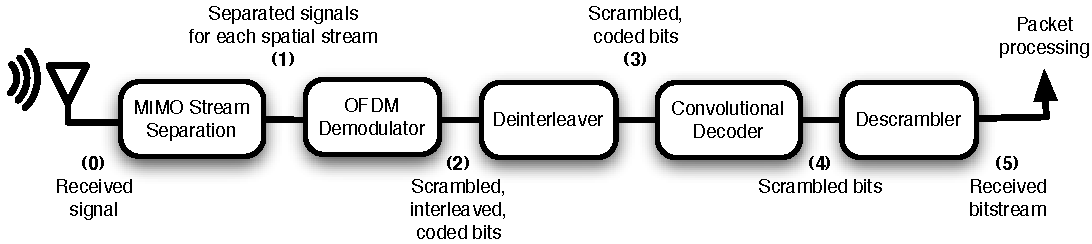
\includegraphics[width=6in]{figures/esnr/mimo_ofdm_decoding_process.pdf}
\caption[The 802.11n MIMO-OFDM decoding process]{\label{fig:ofdm_decoding} The 802.11n MIMO-OFDM decoding process. The MIMO receiver separates the RF signal~(0) for each spatial stream~(1). Demodulation converts the separated signals into bits~(2). Bits from the multiple streams are deinterleaved and combined~(3) followed by convolutional decoding~(4) to correct errors. Finally, scrambling that randomizes bit patterns is removed and the packet is processed~(5).}
\end{figure}

\heading{802.11n Packet Simulator.}
I wrote a custom 802.11a/g/n packet simulator in a combination of MATLAB and the MIT C++ GNU Radio code for SoftRate. Given the CSI describing  a particular wireless channel, the simulator implements packet reception as shown in \figref{fig:ofdm_decoding}. This includes demodulation for BPSK through 64-QAM, deinterleaving, and convolutional decoding with soft inputs and soft outputs. Packets are correctly received when there are no uncorrected bit errors, or else they are lost. Thus given a measured CSI trace, the packet simulator computes which MCS combinations would successfully deliver packets for each CSI record in the trace.

The physical-layer feedback values are computed by the packet simulator. While applying error correction decoding to the received bitstream, the simulator also computes SoftRate's soft-output BER estimate for each CSI record and for each SISO rate. The simulator also computes the Effective SNR values for each CSI, but to reflect real-world NIC limits, Effective SNR is not given the measured CSI. Instead, I corrupt the CSI at the level of ADC quantization. This typically induces an error of $\pm$1.5\dB in the output Effective SNRs.

\heading{802.11n MAC Simulator.}
A second component of the simulator implements the 802.11n MAC. This includes randomized backoff and link-layer packet aggregation. Initially, the simulator is reset to time 0 with default parameters for the MAC protocols, and then a rate selection algorithm will choose a rate for the next transmission. The simulator calculates whether that transmission is received, updates its internal MAC state, and then returns information about packet delivery to the rate control algorithm, as well as the appropriate physical-layer feedback. After every transmission, the simulator executes 802.11n's randomized backoff process and computes the new time for the start of the next transmission.

In 802.11n, transmitters send aggregated packet batches up to 65,000 bytes long. Batches are shortened for slower rates, when the transmission time is instead limited by the 802.11n standard's 4\ms restriction on transmission duration. Given an MCS, the simulator computes how long the transmission will last, then whether the batch is received successfully. As a single packet batch transmission can last up to 4\ms, this may overlap multiple channel probes in the trace. As senders use a fixed MCS for the entire transmission, the MAC simulator requires that $\geq$80\% of simulated packets for those channel records be received correctly in order for the batch to be received (this allows for the effects of coding).

SoftRate operates using the 80th percentile soft estimate from the range of packets. The Effective SNR feedback for a particular packet batch is given from the CSI of the first measurement overlapping that transmission. This models a varying channel that samples for CSI periodically, as happens when CSI is measured during the packet preamble.

\heading{Rate Selection Algorithms.}
The SampleRate, SoftRate, and Effective SNR algorithms are implemented as described previously, and get their inputs and outputs from the packet and MAC simulator components. Each algorithm chooses a rate based on its internal state, and the simulator returns whether the rate succeeds as well as any physical layer feedback, namely SoftRate's BER estimates and the Effective SNR values, measured during the transmission.

\heading{Metrics.}
The goal is to evaluate the ability of these algorithms to respond to changing channel conditions. Thus, the primary metric is the delivered MAC layer rate per time, modeling a UDP application. Higher-layer factors, such as TCP reactions to loss, will affect how this rate translates to throughput. These effects are ignored in the results presented here.

The results reported are the median of five trials where the simulator is initialized with different random seeds. To vary mobility, I scale the trace at different speeds; for example, 4$\times$ mobility means that the records are assumed to arrive 4$\times$ faster than they were measured.

\section{SISO Rate Adaptation Results}
I first examine the performance of Effective SNR for selecting SISO rates. The goal of this experiment is to establish a reasonable baseline, showing that Effective SNR performs as well or better than existing well-studied SISO rate adaptation algorithms, while using a simpler algorithm. If so, this will provide initial validation that the accurate packet delivery predictions provided by my Effective SNR model are useful in practice.

\subsection{Effective SNR vs. Optimal}
I begin by comparing Effective SNR performance against the Optimal algorithm. \figref{fig:siso_rate_time_opt_eff} shows the rate over time for Effective SNR and Optimal over the SISO trace. The rate is averaged over a window of 200\ms to smooth the data for readability. Effective SNR performs excellently. It is below Optimal but consistently tracks the Delayed Optimal algorithm, a realistic upper bound. Overall, Effective SNR delivers 90\% of packets, with about 10\% over-selection of rates.

\begin{figure}[htbp]
      \centering
      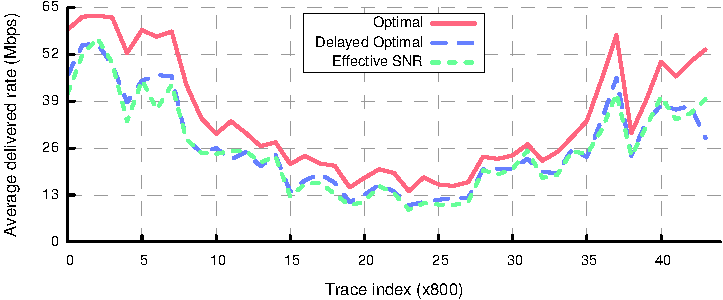
\includegraphics[width=\textwidth]{figures/rate/siso_rate_time.pdf}
      \caption[Effective SNR SISO performance versus Optimal in human-speed mobility]{\label{fig:siso_rate_time_opt_eff} Effective SNR SISO performance versus Optimal in human-speed mobility.}
\end{figure}


Note that Packet SNR was observed to fare quite poorly in mobile channels~\cite{Vutukuru_SoftRate}. Since Effective SNR reflects link fading, its estimates are more accurate (\chapref{chap:delivery}) and are stable (2$\times$--3$\times$ less variance).

%Note this is much better than trained SNR techniques~\cite{Vutukuru_SoftRate}, because packet SNR primarily reflects strong subcarriers, while Effective SNR reflects actual performance and is hence more stable.

\begin{figure}[t]
      \centering
      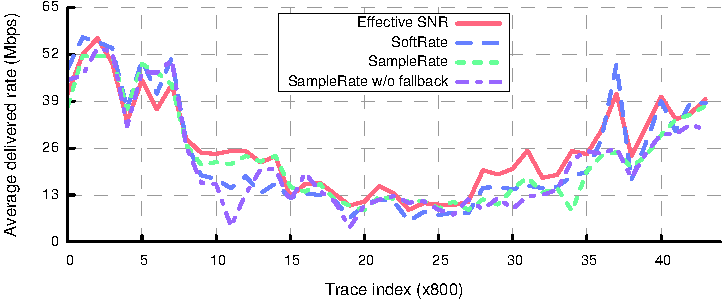
\includegraphics[width=\textwidth]{figures/rate/siso_rate_time_all.pdf}
      \caption[SISO algorithm performance in human-speed mobility]{\label{fig:siso_rate_time_opt_eff_sr_so} Effective SNR, SoftRate, and SampleRate SISO performance in human-speed mobility.}
\end{figure}
\begin{figure}[t]
      \centering
      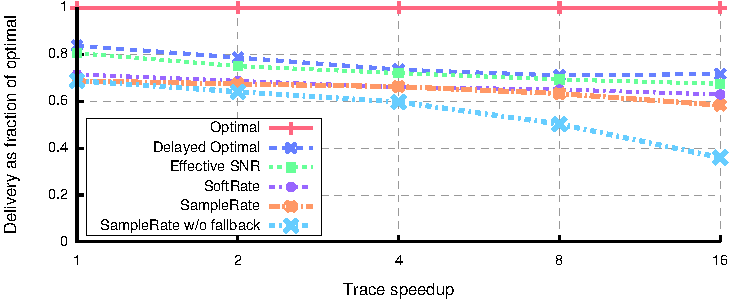
\includegraphics[width=\textwidth]{figures/rate/siso_rate_skip_ratio.pdf}
      \caption[SISO algorithm performance in fast mobile channels]{\label{fig:siso_rate_skip_opt_eff_sr_so} OPT, Effective SNR, SampleRate, and SoftRate SISO performance in fast mobile channels.}
\end{figure}

\subsection{Effective SNR vs. 802.11a/g algorithms}
Next, I compare Effective SNR with SampleRate and SoftRate, in order to see how it performs against current state-of-the-art SISO rate adaptation algorithms.

\figref{fig:siso_rate_time_opt_eff_sr_so} shows the delivered rate of each algorithm versus time. While it is hard to separate the lines on the graph, at 1$\times$ speed, Effective SNR slightly outperforms SoftRate, which slightly outperforms SampleRate. These results were surprising, because the SoftRate work~\cite{Vutukuru_SoftRate} indicated a large gap between SoftRate and SampleRate. In deeper analysis, I discovered that reducing the rate for retries is an important factor that gives SampleRate short-term adaptability. Without this rate fallback (the ``SampleRate without fallback'' line), SampleRate loses 25\%--50\% of its performance in mobile channels (\figref{fig:siso_rate_skip_opt_eff_sr_so}). This variant without fallback is the SampleRate algorithm that was the basis for earlier comparisons.\footnote{M. Vutukuru, personal communication, and code inspection.}

\figref{fig:siso_rate_skip_opt_eff_sr_so} shows the effects of mobility on SISO channels. Each line plots the total amount of data delivered during the trace as a function of the speed at which the trace is played. The speeds range from $1\times$ to $16\times$, corresponding to movement speeds of between walking speeds $\approx$3\mph when using the normal simulation, to about 50\mph for the fastest playback. The $y$-axis value is normalized by the Optimal algorithm's performance to better illustrate how the relative performance changes at different speeds.

This plot shows that all schemes fall off with increased speed; the gap between Optimal and the Delayed Optimal algorithm increases from about 20\% to about 30\% at the fastest speeds. However, even in these mobile channels, Effective SNR holds up quite well and tracks the Delayed Optimal algorithm within 5\%.

SoftRate performs slightly worse at the normal human speeds, but maintains a nearly constant performance, about 70\% of Optimal, as the trace speed increases. SampleRate degrades the fastest with increasing mobility, and the version that does not reduce rate on retries finally less than 40\% of the Optimal performance, while the other algorithms maintain better than 60\% of Optimal performance at all speeds.

Finally, I note that while the performance differences between the schemes can be significant, other evaluations have reported larger differences. Note that they studied throughput based on TCP traffic, which will magnify performance gaps by reacting to packet loss. The UDP-like results I generated using my simulator capture the underlying accuracy of the individual schemes instead.

\begin{figure}[t]
      \centering
      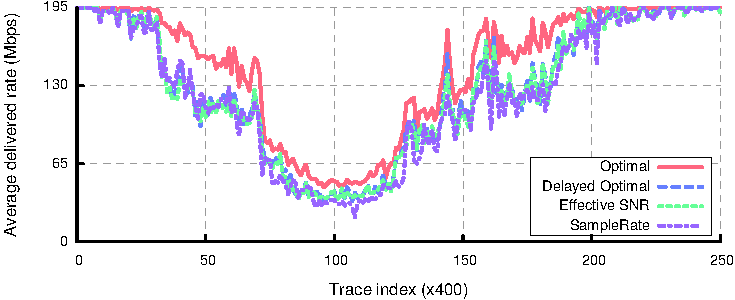
\includegraphics[width=\textwidth]{figures/rate/mimo_rate_time.pdf}
      \caption[MIMO algorithm performance in human-speed mobility]{\label{fig:mimo_eff_snr_time} Optimal, Effective SNR, and SampleRate MIMO performance in human-speed mobility.}
\end{figure}

\begin{figure}[ht]
      \centering
      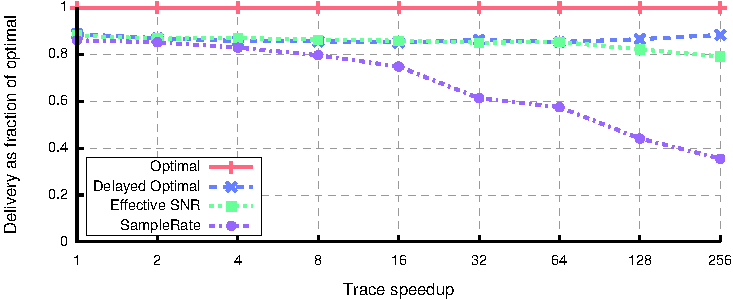
\includegraphics[width=\textwidth]{figures/rate/mimo_rate_skip_ratio.pdf}
      \caption[MIMO algorithm performance in fast mobile channels]{\label{fig:mimo_eff_snr_speedup} Optimal, Effective SNR, and SampleRate MIMO performance in faster mobile channels.}
\end{figure}

\section{MIMO Rate Adaptation}
Now I extend the evaluation to MIMO channels. This will show the generality of my model, which can flexibly support multiple spatial streams. I compare Effective SNR to an 802.11n-enabled version of SampleRate, to understand whether the larger search space will increase the performance gap between the two schemes.

\figref{fig:mimo_eff_snr_time} and \figref{fig:mimo_eff_snr_speedup} show the performance of an unmodified Effective SNR algorithm selecting among 802.11n MIMO rates, as well as (modified) SampleRate and the two Optimal algorithms. This graph does not include a line for SoftRate, as it is not defined for multiple streams.
%\figref{fig:mimo_eff_snr_time} and \figref{fig:mimo_eff_snr_speedup} show the rate versus time and rate versus speedup graphs. 
These figures are in the same form as for SISO, except the range of rates has grown by a factor of 3 to support up to 195\Mbps. The MIMO trace is longer and has more packets-per-second, and thus includes enough data to speed up the trace by a factor of up to 256$\times$.

Overall, the Effective SNR trends in these graphs are similar to those in the SISO graphs. At human mobility speeds, Effective SNR tracks the Delayed Optimal algorithm and delivers excellent performance, with 75\% accuracy and 10\% over-selection. In faster mobile channels, Effective SNR tracks the Delayed Optimal algorithm until the speeds increase to about 128$\times$, after which there is a slightly larger gap with for MIMO than for SISO. This arises likely because Effective SNR must now choose between 24 rates instead of 8. It is slightly more likely to choose rates lower than the highest rate that would have worked.

These graphs also show that---as with SISO links---SampleRate performs well in human speed mobility, only slightly worse than Effective SNR. But for SampleRate, this trend \emph{does not hold}, and as the speed of the trace gets faster the performance degrades rapidly to around one-third of Optimal, and less than half of Effective SNR. The difference between SampleRate and Effective SNR highlights that Effective SNR is able to handle the large MIMO rate space even in rapidly-changing channels, while the probe-based SampleRate algorithm cannot.

%Finally, note that with three antennas there are only four two- and three-stream rates over 117\Mbps (130, 156, 175.5 and 195 Mbps). The visible gap between indices 25--50 in \figref{fig:mimo_eff_snr_time} reflects only the difference between 1 or 2 rates of potentially different antenna modes. Taken together, these results imply that Effective SNR's MIMO performance is highly competitive.


\section{Enhancements: Transmit Antenna Selection}
I conclude this chapter with an example that highlights the strength of my Effective SNR in that it accommodates choices other than just rate. In particular, I amended the implemented Effective SNR algorithm to select the best transmit antenna set.

Transmit antenna selection can be useful in practice, for instance in an 802.11n AP that selects which antennas to use to send packets to a legacy 802.11a/g client (plus uses all antennas to receive packets). With three antennas to choose from, the expected theoretical gain in SNR is a little over 2.5\dB~\cite{Goldsmith}. For a SISO link, this gain is likely enough to advance to a higher rate.

I ran my antenna selection-enabled Effective SNR algorithm on a 3x1 MISO channel, extracted from the 3x3 MIMO trace. These measurements correspond to those that would be measured if the transmitter exploited the ``extension spatial streams'' CSI probe to measure the 3x1 MISO channel as I described in \secref{sec:csi_collection}.

Using the MISO CSI feedback, the Effective SNR algorithm chose the antenna with the highest Effective SNR for the next transmission. This gave a gain in the total packet delivery of 5\%. For comparison, the Optimal antenna selection algorithm achieved a 10\% increase by always knowing which antenna was best.

While transmit antenna selection presents a relatively small gain for this trace, it comes at no cost and does not complicate the Effective SNR algorithm. In contrast, no other rate adaptation schemes as directly support these enhancements. They would instead require customized, multi-dimensional probing algorithms and coarse adaptation of antennas to implement antenna selection.

Antenna selection is one of many ways that my Effective SNR model can be applied beyond simple rate selection. In the next chapter, I present a study of four different network configuration applications.

\section{Summary}
In this chapter, I presented a detailed evaluation of Effective SNR in the context of configuring the rate for 802.11a/g and 802.11n links in a mobile setting. The results for the single-antenna 802.11a/g systems showed that Effective SNR performs as well as or better than existing state-of-the-art algorithms for rate adaptation, with a much simpler rate selection algorithm.

A key result of this evaluation is that this good performance extends to 802.11n, while the probe-based SampleRate algorithm suffered in the larger search space. This validates my fundamental claim that probe-based algorithms will suffer in large search spaces with dynamic channels, and it motivates the need for and benefits of my Effective SNR approach.

Finally, I also showed that Effective SNR easily supports additional enhancements such as antenna selection. In the next chapter, I will flesh out Effective SNR applications by applying my model to a set of other configuration problems along different dimensions of the configuration space.

%%%%%%%%%%%%%%%%%%%%%%%%%%%%%%%%%%
\ifx\mainfile\undefined
%
% ==========   Bibliography   ==========
%
%\nocite{*}   % include everything in the uwthesis.bib file
\bibliographystyle{plain}
\bibliography{dhalperi_thesis}

\end{document}
\fi
